%% Exemplo de utilizacao do estilo de formatacao normas-utf-tex (http://normas-utf-tex.sourceforge.net)
%% dúvidas acessar o site acima
%%
%%
%% Autores: (200?-2011) Hugo Vieira Neto (hvieir@utfpr.edu.br)
%%          (200?-2011) Diogo Rosa Kuiaski (diogo.kuiaski@gmail.com)
%%          (2011-2017) Marcos Talau <talau@users.sourceforge.net>
%% Colaborador:
%%          (2011) César M. Vargas Benitez <cesarvargasb@gmail.com>

%%
%% IMPORTANTE: O texto está escrito com acentuação antiga, atualmente você
%%             pode escrever acentos sem precisar de códigos para tal.
%%

\documentclass[openright]{normas-utf-tex} %openright = o capitulo comeca sempre em paginas impares
%\documentclass[oneside]{normas-utf-tex} %oneside = para dissertacoes com numero de paginas menor que 100 (apenas frente da folha) 

% force A4 paper format
\special{papersize=210mm,297mm}

\usepackage[alf,abnt-emphasize=bf,bibjustif,recuo=0cm, abnt-etal-cite=2, abnt-etal-list=99]{abntcite} %configuracao correta das referencias bibliograficas.

\usepackage[brazil]{babel} % pacote portugues brasileiro
\usepackage[utf8]{inputenc} % pacote para acentuacao direta
\usepackage{amsmath,amsfonts,amssymb} % pacote matematico
\usepackage{graphicx} % pacote grafico
\usepackage{times} % fonte times
\usepackage[final]{pdfpages} % adicao da ata

%Podem utilizar GEOMETRY{...} para realizar pequenos ajustes das margens. Onde, left=esquerda, right=direita, top=superior, bottom=inferior. P.ex.:
%\geometry{left=3.0cm,right=1.5cm,top=4cm,bottom=1cm} 

% ---------- Preambulo ----------
\instituicao{Universidade Tecnológica Federal do Paraná} % nome da instituicao
\programa{DEPARTAMENTO ACADÊMICO DE ELETRÔNICA } % nome do programa
\area{ESPECIALIZAÇÃO EM INTERNET DAS COISAS} % [Engenharia Biom\'edica] ou [Inform\'atica Industrial] ou [Telem\'atica]

\documento{Dissertação} % [Disserta\c{c}\~ao] ou [Tese]
\nivel{Pos-graduação} % [Mestrado] ou [Doutorado]
\titulacao{Especialista} % [Mestre] ou [Doutor]

\titulo{{Sistema autonomo de gerenciamento de luzes}} % titulo do trabalho em portugues
\title{\MakeUppercase{Self-contained lighting management system}} % titulo do trabalho em ingles

\autor{Luis Denis Pliskievski de Lara} % autor do trabalho
\cita{LARA, Luis Denis Pliskievski de} % sobrenome (maiusculas), nome do autor do trabalho

\palavraschave{IOT, nodeMCU, ESP8266, energia, controle, autonomo} % palavras-chave do trabalho
\keywords{IOT, nomeMCU, ESP8266, energy, contro, self-contained} % palavras-chave do trabalho em ingles

\comentario{\UTFPRdocumentodata\ apresentada ao \UTFPRprogramadata\ da \ABNTinstituicaodata\ como requisito parcial para obtenção do grau de ``\UTFPRtitulacaodata\ em Intenet das Coisas Área de Concentração: \UTFPRareadata.}

    \orientador{Glauber Brante} % nome do orientador do trabalho
%\orientador[Orientadora:]{Nome da Orientadora} % <- no caso de orientadora, usar esta sintaxe
%\coorientador{Nome do Co-orientador} % nome do co-orientador do trabalho, caso exista
%\coorientador[Co-orientadora:]{Nome da Co-orientadora} % <- no caso de co-orientadora, usar esta sintaxe
%\coorientador[Co-orientadores:]{Nome do Co-orientador} % no caso de 2 co-orientadores, usar esta sintaxe
%\coorientadorb{Nome do Co-orientador 2}	% este comando inclui o nome do 2o co-orientador

\local{Curitiba} % cidade
\data{\the\year} % ano automatico

% desativa hifenizacao mantendo o texto justificado.
% thanks to Emilio C. G. Wille
\tolerance=1
\emergencystretch=\maxdimen
\hyphenpenalty=10000
\hbadness=10000
\sloppy

%---------- Inicio do Documento ----------
\begin{document}

\capa % geracao automatica da capa
\folhaderosto % geracao automatica da folha de rosto

% Lembre-se de que a ficha catalografica eh impressa no verso da folha de rosto
% Ficha catalografica
\fichacatpum{T137}
\fichacatautor{Lara, Luis Denis Pliskievski de}
\fichacatpgbib{\pageref{bibstart}-\pageref{bibend}}
\fichacatpalcha{1. Intenet das coisas. 2. Redes de comutadores. 3. TCP/IP (Protocolo de rede de computação), ...}
\fichacatpdois{CDD (22. ed.) 621.3}
\fichacatbib{Biblioteca xxxxxx}
\fichacat

% insercao da ATA
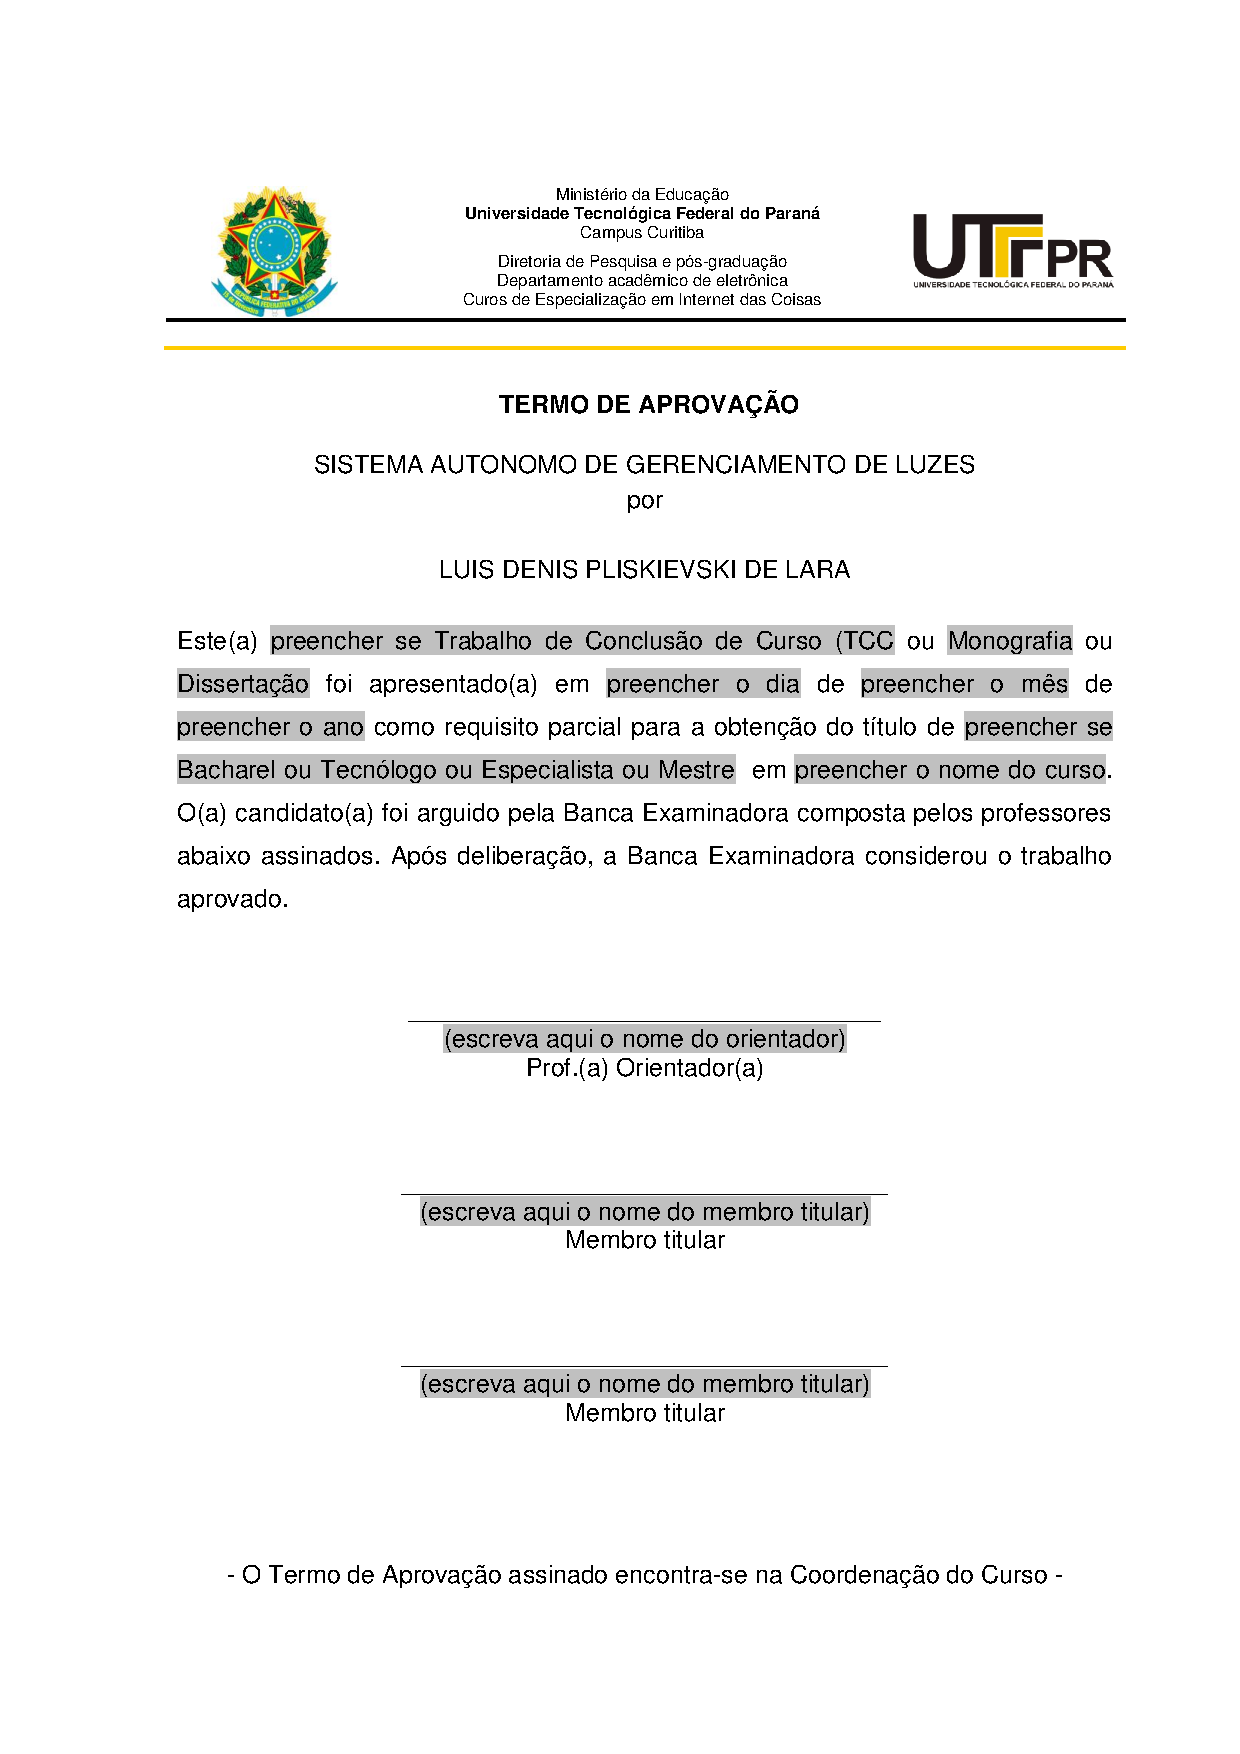
\includepdf{termo.pdf}

% dedicatoria
\begin{dedicatoria}
Dedico esse trabalho em memória de minha mãe que sempre me incentivou a buscar mais conhecimento.
\end{dedicatoria}

% agradecimentos (opcional)
\begin{agradecimentos}
A todos que de alguma forma me apoiaram na trajetoria, não deixaram eu desistir e mais do que nunca acreditaram em mim em momentos que eu dúvida da minha capacidade.
Agradeço ao meu colega Konrado Biernet por me ajudar a desenvolver esse trabalho e a minha namorada Aline Frassato, por compreender os tempos que tive que deixa-la sozinha.
\end{agradecimentos}

%resumo
\begin{resumo}
Essa dissertação mostra de forma pratica o uso da internet da coisas para buscar eficiência no uso de recursos energicos voltados para gerenciamento de luz, aonde hoje temos um gasto substâncial e muitas vezes mal administrado.
\end{resumo}

%abstract
\begin{abstract}
This dissertation shows in a practical way the use of the internet of things for the search of efficiency in the use of energy resources directed to the management of light, and today we have a specific and often mismanaged expense.
\end{abstract}

% listas (opcionais, mas recomenda-se a partir de 5 elementos)
%\listadesiglas % geracao automatica da lista de siglasp
% sumario
\sumario % geracao automatica do sumario


\setcounter{page}{12}

%---------- Primeiro Capitulo ----------

\chapter{Introdução}


Com o advento da internet e evolução, temos a possibilidade de criar dispositivos inteligentes \cite{Novatec} para nos auxiliar em situações corriqueiras, como controle de acesso, controle de frotas, gerenciamento de energia e água.

Nesse trabalho iremos desmostrar um sistema inteliganete de gerenciamento de luzes para comercio, empresas e mesmo casas.

Para o desenvolvimento do recurso usaremos os itens:

\begin{itemize}
       	\item ESP8266 - NomeMCU V3
        \item Sensor de corrente Allegro ACS712 (ACS712ELCTR-30A-)
        \item Servidor MQTT
        \item Sensor de presença PIR DYP-ME003
\end{itemize}
\section{Motivação}

Há um grande disperdício de energia em corporações e lojas devido  a falta de controle sobre o consumo de energia o que em analise calculista pode representar um impacto as contas da empresa e ao meio ambiente, pois hoje falamos muito em eficiente energética e isso pode trazer efeitos signiticativos para administração das empresas.

\section{Objetivos}

\subsection{Objetivo Geral}

O objetivo prinicipal é demonstrar e gerenciar o consumo de energia sobre fontes de iluminação visando diminuir o consumo e aumentar a eficiência do uso dos recursos energéticos. 

\subsection{Objetivos Específicos}

\begin{itemize}
	\item Controlar o consumo de energia.
	\item Representar por meio de números o consumo real. 
	\item Melhorar o consumo energético através de gerenciamento autonomo.
	\item Entregar uma previsão de consumo x gasto mensal.
\end{itemize}


%---------- Segundo Capitulo ----------
\chapter{Desenvolvimento}
\label{chap:desenv}

 
Para o desenvolvimento do projeto foi utilizando as  linguagens c++   \cite{Altabooks} e HTTP.

Durente o processo de desenvolvimento previmos a nomeação do módulo durante a primeira inicialização, após a configuração do SSID e senha da rede.

Com a rede configurada o nó começa a enviar dados da para um servidor MQTT   \cite{Novatec} para ser tratado no painel de gerenciamento. 

\section{NodeMCU}
Optei pelo uso do microcontrolador ESP8266, presente no módulo NODEMCU, que possui as seguites caracteristas:
\begin{itemize}
    \item Certificação WIFI Alliance;  \cite{espressif}
    \item Protocolos 802.11 b/g/n;\cite{espressif}
    \item CPU Tensilica L106 32-bit processor (80MHz ~ 160MHz )  \cite{Novatec}
    \item 4MB de armazenamento;
    \item Suporte aos modos Station/SoftAP/SoftAP+Station;\cite{espressif}
    \item Autenticação WPA/WPA2 com encriptação WEP/TKIP/AES;\cite{espressif}
    \item Supoter atualização OTA;\cite{espressif}
    \item Procolocolos de Rede IPv4, TCP/UDP/HTTP;\cite{espressif}
\end{itemize}

Durante o processo de desenvolvimento do projeto foi encontrado uma limitação do uso de vários nós em rede MASH, pois há um limite de conexões simultaneas permitidas, ou seja se mais 5 nós tentarem se manter conectados a um NodeMCU a conexão mais antiga será derrubada, podendo gerar assim algumas falhas de tramissão de dados. 

Pois isso optei em não usar a rede MASH e manter todos os nós comunicando diretamente com o servidor MQTT.

Caso a rede esteja indisponível por alguma motivo o nó poderá armazenar informações em sua memória de até 7 dias.

\section{Sensor de corrente Allegro ACS712}
O medidor de corrente Allegro ACS712  \cite{Allegro} pode trabalhar com correntes de -30A à +30A   \cite{Allegro} amperes, mais que suficiente para os padrões que usamos em estrutura de iluminação, aonde as correntes geralmente não são maiores que 10A.

A taxa de amostragem durante o desenvolvimento deve um pequena diferença comparando com o resultado de multimetro. Essa diferença ficou entre 55mA e 70mA. Isso acontece devido ao ruído do L106 e o ruído do próprio Allegro ACS712.

Para calular o consumo utilizamos algumas informações do padrão brasileiro, como a taxa de amostragem de 60Hz de nossas redes. Com base nessas informações e utilizando a biblioteca EmonLib, a biblioteca originalmente foi desenvolvida para Arduíno mas é compatível com o ESP8266 utilizado.

Uma vez realizada a medição os dados são enviados via MQTT   \cite{Novatec}para serem exibidos no front-end.

\section{Sensor de presença PIR DYP-ME003}

Também utilizamos um sensor de presença modelo PIR DYP-ME003   \cite{openimpulse}
para ter um controle automatico de uso de salas. 

Com isso no momento que a pessoa entra da sala o sensor envia um sinal que acende as lampadas automaticamente e começa a bilhetagem das luzes naquela sala.


\section{Firmware}

O firmware foi desenvolvimento utilizando liguagem c++. Os principais item que de trabalho do firmware são:


\begin{itemize}
    \item Primeira Inicialização e configuração primaria;
    \item Gerenciador de funções;
    \item Atualização OTA;
\end{itemize}

O firmware foi divido em 3 etapas para facilitar o entendimento do funcionamento básico do mesmo, mas tempo real é executado somente um binário dentro do dispositivo.

Todas as mensagens trocas entre nó e servidor são no formato JSON  \cite{json-devmedia}.

Como no exemplo abaixo:
\begin{center}
\textit
sensor\{\\ 
status: boolena; \\
dimmer: int16;\\
Consumo:int16; \\
grupo:string;\\
laststate: booelan;\\
Hearbeat: date: \\
PresenceSensor:boolean:\\
\}
\end{center}


\subsection{Primeira Inicialização e configuração primaria}
Para a primeira inicialização do nó o rádio será setado como AP e terá um servidor DHCP para fornecer 2 IP's classe C.
Com isso podemos utilizar um notebook ou smartphone para abrir a página de configuração do nó.

Internamento foi criado um servidor WEB com acesso via porta 80 e a uma página HTTP que será utilizada para configurar esses dados de forma simples e clara, pois a página não terá aba ou outras páginas para navegar.

Na página de configuração poderes setar as seguintes opções:
\begin{itemize}
    \item Nome do nó;
    \item Grupo do nó;
    \item Nome da Rede;
    \item Senha de acesso;
    \item Tipo de autenticação e padrão criptografia;
    \item Habilitar ou desabilitar o acesso via SSH;
\end{itemize}

Para em caso de falha na configuração ou qualquer outro problema temos um botão de reset através de uma GPIO  \cite{Elsevier}. com isso o firmware retorna o estado de fábrica, podemos assim realizar todo o processo de configuração novamente.

\subsection{Gerenciador de funções}

Para o gerenciamento utilizamos um serviro MQTT para troca das mensagens entre nó e a plataforma de gerenciamento. 

O firmware ao receber uma mensagem da plataforma verifica a qual grupo perterce, que no caso pode ser do tipo:

\begin{itemize}
    \item Acender/Apagar luz;
    \item Estado na Luz;
    \item Controlar intensidade da Luz;
    \item Consumo;
    \item Verificar grupo;
    \item Trocar de grupo;
    \item Respostas autônomas;
\end{itemize}

\subsubsection{Acender/Apagar luz}
Para a função interação de acender e apagar a luz trabalhamos com o estado do bit, no caso 0 e 1 aonde:

\begin{itemize}
    \item O Apaga a luz;
    \item 1 Acende a luz;
\end{itemize}

Esse processo é simples de ser realizado e ao executar com sucesso o comando é enviado uma resposta de ACK para o gerenciador remoto, caso contrário o mesmo receberá um NACK.

\subsubsection{Estado na Luz}

Essa é uma função de retorno de status do nó para o gerenciador remoto. Nessa função pegamos o status da lampada, acessa ou apagada e retornamos de forma binária para o servidor.

\subsubsection{Controlar intensidade da Luz}
Nesse caso utilizamos a mesma função de Acender ou Apagar a luz, mas verificamos se a mensagem recebida é maior que 0 e menor 99, caso seja verdade pegamos o valor recebido e aplicamos como porcentagem sobre 100\% de forma a adequar a intensidade da luz do nó especifico.

\subsubsection{Consumo}
Para a função de consumo, pegamos o valor do ponteiro double e retornamos para o servidor remoto.

Esse valor só é zerado no momento que o nó é desligado, nesse momento o valor é enviado o servidor para ser inserida no banco de dados e consumida pelo gerenciador remoto.

\subsubsection{Verifica grupos}

Ao receber uma mensagem nessa função, o mesmo irá verificar se é pertecendo ao grupo e retornará as seguintes informações:

\begin{itemize}
    \item Valor estado;
    \item Valor dimmer;
    \item Valor Consumo;
    \item Grupo;
    \item Ultimo estado;
    \item Data-hora do nó;
    \item Valor sensor de presença;
\end{itemize}

\subsubsection{Trocar de Grupo}
Ao receber a mensagem para trocar de grupo o nós irá verificar o nó o mesmo está e se for o valor recebido for diferente do atual, ele irá armazenar o valor atual em um arquivo interno e atualizar o valor para o novo grupo recebido, enviando em seguida uma mansagem de ACK para o servidor remoto, caso não seja executado o comando ele retornará um NACK par o servidor.

\subsubsection{Respostas autônomas}
O nó em cada ação recebida via MQTT ou GPIO, o nó envia uma mensagem para servidor com os seguintes dados;

\begin{itemize}
    \item Nome do nó;
    \item IP do nó;
    \item Mascará de rede;
    \item gateway padrão;
    \item Valor estado;
    \item Valor dimmer;
    \item Valor Consumo;
    \item Grupo;
    \item Ultimo estado;
    \item Data-hora do nó;
    \item Valor sensor de presença;
    \item Tempo em atividade;
    \item Versão do firmware;
\end{itemize}

\subsection{Atualização OTA}

O ESP8266 suporta atualização de firmware via rede wireless  \cite{espressif}, sendo assim não é preciso conectar um cabo usb para realizar o processo no mesmo. 
Pensando nessa funcionalidade crei uma função para receber o firmeare a fazer a atualização.

Ao receber a mensagem de atualizaçao disponível é comparada a versão local com a nova versão disponível, caso seja diferente o nó conecta-se a um repositorio e baixa o novo arquivo, uma vez realizado a cópia, ele verificar a integridade através de uma comparação entre o MD5 do servidor com o MD5 do arquivo local, se a combinação for igual, então para os serviços, atualiza o binário e reinica os serviços novamente.
Após a atualização do firmware não é necessário reconfigurar o nó, pois as configurações são salvas em uma parte segregada da memória, fazendo isso um processo limpo do binário. 


%---------- Terceiro Capitulo ----------
\chapter{Conclusão}

Vemos que a utilizaçao dos recursos de internet das coisas podem nos ajudar no gerenciamento de energia, como nesse caso aplicado a luzes, mas podendo ser ampliado para qualquer cénario que utilize energia elétrica como recurso principal.

Com o uso controlado podemos ter uma maior eficiência e diminuição de gastos, fazendo assim uma solução verde e amiga dos recursos naturais.



%---------- Referencias ----------
\clearpage % this is need for add +1 to pageref of bibstart used in 'ficha catalografica'.
\label{bibstart}
\bibliography{reflatex} % geracao automatica das referencias a partir do arquivo reflatex.bib
\label{bibend}

% --------- Ordenacao Afabetica da Lista de siglas --------
%\textbf{* Observa\c{c}\~oes:} a ordenacao alfabetica da lista de siglas ainda nao eh realizada de forma automatica, porem
% eh possivel se de realizar isto manualmente. Duas formas:
%
% ** Primeira forma)
%    A ordenacao eh feita com o auxilio do comando 'sort', disponivel em qualquer
% sistema Linux e UNIX, e tambem em sistemas Windows se instalado o coreutils (http://gnuwin32.sourceforge.net/packages/coreutils.htm)
% comandos para compilar e ordenar, supondo que seu arquivo se chame 'dissertacao.tex':
%
%      $ latex dissertacao
%      $ bibtex dissertacao && latex dissertacao
%      $ latex dissertacao
%      $ sort dissertacao.lsg > dissertacao.lsg.tmp
%      $ mv dissertacao.lsg.tmp dissertacao.lsg
%      $ latex dissertacao
%      $ dvipdf dissertacao.dvi
%
%
% ** Segunda forma)
%\textbf{Sugest\~ao:} crie outro arquivo .tex para siglas e utilize o comando \sigla{sigla}{descri\c{c}\~ao}.
%Para incluir este arquivo no final do arquivo, utilize o comando \input{arquivo.tex}.
%Assim, Todas as siglas serao geradas na ultima pagina. Entao, devera excluir a ultima pagina da versao final do arquivo
% PDF do seu documento.


%-------- Citacoes ---------
% - Utilize o comando   \citeonline{...} para citacoes com o seguinte formato: Autor et al. (2011).
% Este tipo de formato eh utilizado no comeco do paragrafo. P.ex.:   \citeonline{autor2011}

% - Utilize o comando   \cite{...} para citacoeses no meio ou final do paragrafo. P.ex.:   \cite{autor2011}



%-------- Titulos com nomes cientificos (titulo, capitulos e secoes) ----------
% Regra para escrita de nomes cientificos:
% Os nomes devem ser escritos em italico, 
%a primeira letra do primeiro nome deve ser em maiusculo e o restante em minusculo (inclusive a primeira letra do segundo nome).
% VEJA os exemplos abaixo.
% 
% 1) voce nao quer que a secao fique com uppercase (caixa alta) automaticamente:
%\section[nouppercase]{\MakeUppercase{Estudo dos efeitos da radiacao ultravioleta C e TFD em celulas de} {\textit{Saccharomyces boulardii}}
%
% 2) por padrao os cases (maiusculas/minuscula) sao ajustados automaticamente, voce nao precisa usar makeuppercase e afins.
% \section{Introducao} % a introducao sera posta no texto como INTRODUCAO, automaticamente, como a norma indica.


\end{document}

